\documentclass[12pt, a4paper]{report}
\usepackage[utf8]{inputenc}
\usepackage[swedish]{babel}
\usepackage{relsize}
\usepackage[backend=biber, style=numeric-comp, sorting=none]{biblatex}
\usepackage{csquotes}
\usepackage{graphicx}
\usepackage{titlesec}
\usepackage{titling}
\usepackage{pgf-pie}
\usepackage{hyperref}
\usepackage{csquotes}
\usepackage{fancyhdr}
\pagestyle{fancy}
\lhead{Eddie Englund Gymansiearbete TEINF17A VT 2020}
\rhead{\thepage}
\renewcommand{\headrulewidth}{0.4pt}
\renewcommand{\headheight}{14.999pt}

\setcounter{tocdepth}{3}
\setcounter{secnumdepth}{3}

\emergencystretch=1em

\setcounter{secnumdepth}{0}

\bibliography{bibliography.bib}
\addbibresource{biliography.bib}

\author{Eddie Englund}
\title{Linux vs Windows\\[0.2em]\smaller{}En djupgående analys av prestandaskillnader mellan Microsoft Windows och Manjaro Linux}
\date{VT 2020}

\renewcommand{\abstractname}{Abstract}
\renewcommand{\abstract}{Abstract}
\renewcommand*{\bibfont}{\small}


\begin{document}

\begin{titlepage}
    \maketitle

    \begin{center}
        \thispagestyle{empty}
    
        
\includegraphics[width=0.15\textwidth]{nti}\par\vspace{1cm}

    {\scshape\LARGE NTI Gymnasiet Gärdet \par}
    \vspace{1cm}
    {\scshape\Large Examensarbete, April 2020\par}
	\vspace{1.5cm}
    \textbf{
    Student: Eddie Englund, eddie.englund@elev.ga.ntig.se även eddie.englund@protonmail.com}
    \vspace{0.2cm}

    Handledare NTIG: Haris Kasumović, Haris.Kasumovic@ntig.se
    \vspace{0.1cm}

    Examinator NTIG: Haris Kasumović, Haris.Kasumovic@ntig.se
    
    \end{center}
\end{titlepage}


\section{Sammanfattning}\label{sum}

    \begin{abstract}

    \end{abstract}

\tableofcontents

\vspace{3cm}

    
\section{Inledning}
 
 
   I och med att världen blir mer och mer digitaliserad för varje dag som går, så är det inte konstigt att det finns en massiv marknad med olika alternativ för nästintill allting i den digitaliserade världen. Allt från telefoner till hemdatorer eller kanske till och med robotdammsugare eller också en robotgräsklippare. Alla dessa digitaliserade mirakel har en sak gemensamt. Dem alla har ett operativsystem.
 
   Världens mest kända operativsystem\cite{winstat} är Microsoft Windows. Microsoft har en lång rad med olika versioner av sitt operativsystem\cite{windows}: Windows XP, Windows Vista, Windows 7[\dots] och deras senaste (och förmodligen sista) operativsystem Windows 10.
    
   Apple har flera olika operativsystem\cite{appleOS} I deras olika produkter. I deras datorer så har man macOS, i deras telefoner har dom IOS och i deras nya Ipads så har dom iPadOS.
    Det finns faktisk ett tredje ``operativsystem''; Linux är en så kallad Kernel \cite{redhat} som är det man kan bygga ett operativsystem på. Linux har många olika operativsystem som är kallade för distributioner eller förkortat \textit{``distros''}. Linux är välkänt. Speciellt inom utvecklarvärlden eftersom att det är mycket vänligt för utvecklingsmiljöer, dessutom så har Linux (oftast) en mycket god prestanda på maskiner med mindre processorkraft\cite{whatislinux}. På grund av detta så är bl.a: iPadOS, IOS, macOS, Android och nästintill allting annat som inte har så mycket processorkraft som t.ex en hiss någon form a Linux som operativsystem.
    
\section{Bakgrund/Teori}


    \subsection{Syfte/Frågeställning}
    Udersökningens syfte är att ta reda på om Linux eller Windows har olika prestanda och varför. Är det så att dom har olika prestana i olika typer av applikationer eller är det konstant? Undersökningen kommer att använda en rad olika tester för att ta reda på om hypotesen är san.
 

    \subsection{Hypotes}

    Utifrån mina egen upplevelse så är Linux (när man väl har konfiguerarat det ordentligt) en mycket mer stabil och snabbare upplevelse en Windows 10.
 

    \subsection{Linux}
 
   Linux är inte operativsystem. Däremot, så är Linux det som kallas för en ``kernel''\cite{redhat}. Det är hjärtat av operativsystemet eller kanske lite bättre jämfört med hjärnan av operativsystemet. Kerneln är en typ av mellanhand, mellan mjukvaran och hårdvaran. Den hanterar minnet, olika typer av processer, drivrutiner, systemanrop och säkerhet.
 

    \subsubsection{Distributioner}

   Eftersom att Linux är en kernel så finns det många så kallade distributioner/versioner (operativsystem). Skillnaderna på dem olika distributionerna kan variera högt, oftast handlar dem största skillnaderna om vilka så kallad ``repositories'' (arkiv med mjukvara) man använder för att distribuera mjukvara. Dessutom så kan det handla om vilka filsystem man använder men också hur mycket eller hur lite förinstallerade program som finns när man installerar distributionen.

   \subsubsection{Repositories}

    En högt definerande egenskap hos Linux är användandet av ``repositories''. Repositories är arkiv eller data banked med mjukvara. Man använder sig utav dessa för att lättare och säkert installera program.

    Normalt sätt när man ska installera ett program på Windows eller Mac så öppnar man en webbläsare och söker på mjukvaran man vill ha, går till sidan, laddar ner en program installatör för det programmet man vill ha, sedan kör man den. Efter det kan man ta bort installören, om man kommer ihåg det.
    
    Men inte på Linux. På Linux så använder man offtast sig av en terminal och ett kommando (detta varierar på distron).
    På Manjaro som är Arch baserad så använder man sig utav pacman\cite{pacman}. Pacman är en ``package manager''\cite{pkgmanager}. Den hanterer paket (mjukvara) som man vill ta bort, installera eller kanske uppdatera.

    För att installera ett programm på Manjaro så skulle man skriva: sudo pacman -S programnamn. 

    \small{notera att det går att installera programm på andra sätt}


    \subsubsection{Absolut kontroll}

   En annan fördel med Linux är att man har absolut kontroll. Man kan byta så kallade \textit{window managers} eller förkortat \textit{wm}\cite{wm}. Man kan även göra om Linux kerneln ifall man vill göra något specifik eller kanske inte behöver bitar av den för att optimasera sin maskin. Detta är mycket vanligt inom låg processor kraftiga maskiner som hissar eller smart klockor.

   Allt detta är tack vare att Linux har en öppen källkod och tillåter använda att göra vad dom vill med det. Detta skulle alldrig vara möjligt på Windows eller Mac (om man inte crackar/gör illegala saker) eftersom att deras licenser säger att man inte får och dessutom så får man inte distribuera sina ändringar ifall man har gjort dem.

   \subsubsection{Öppen källkod}


   Den största skillnaden mellan Linux och Windows är att Linux inte är proprietär och har öppen källkod vilket betyder att vem som helst kan bidra med kod för att; göra kerneln eller distributionen bättre och lägga till fler användbara funktioner, men även också att fixa buggar. Öppen källkod har även en annan fördel och det är att koden oftast inte är så kallad \textit{``bloated''}, alltså att det finns kod eller funktioner som inte behövs eller att kod kvaliteten inte är bra. Detta leder till att prestandan på Linux är mycket hög.
    \vspace{1cm}
   Den distributionen som jag har valt att använda är Manjaro\cite{manjaro}. Manjaro är en så kallad \textit{Arch based distro}. Den är baserad på en annan distro som heter Arch Linux som ofta blir kallat för den bästa distron. Däremot så gör Manjaro det lättare att komma igång och så har Manjaro dem flesta fördelarna som Arch Linux har.

   \subsection{Windows}


    \subsubsection{Skrivet I flera språk}
    
    Windows 10 är skrivet i programmeringspråket C\# som är skapat av Microsoft\cite{c}. Microsoft skapade C\# 20 år sedan (2000) när dom ville skriva delar av Windows XP i Java men det fick dem inte eftersom att Oracle sa nej. Så dom utväcklade vad Klaus och Angelika Langer sa i en blog post att ``Java and C\# are almost identical programming languages. Boring repetition that lacks innovation''.\cite{cquote}  
    

    \subsubsection{Proprietärt}
    Windows är också ett operativsystem som är skrivet helt ``in house'' (det är inte öppen källkod).
    Eftersom att det inte är öppen källkod så vet vi inte riktigt va Windows faktiskt håller på med i bakgrunden. Det gör så att man inte kan ändra på saker lika mycket som man kan på Linux. Dessutom så gör det att Microsoft kan göra lite vad det vill eftersom att det inte måste informera sina användare om alla ändringar (om inte lagen kräver det). Dessutom så är Windows ganska restriktivt i och med att man inte har absolut kontroll över bl.a när man ska/vill uppdatera.


   Det så finns det faktiskt en fördel med att inte ha öppen källkod. Microsoft kan skapa en virtuell monopoli över vissa marknader. T.ex så är Windows (inom pc världen) det bästa operativsystemet att spela på. Det här är eftersom att dom flesta spelen är skapade för att köra på Windows. Det är eftersom att DirectX\cite{directx} finns på Windows men också eftersom att det inte är öppen källkod så är det inte särskillt lätt att piratkopiera spelen och deras innehåll.


 
\section{Metod}
 

\subsection{Språk och program}
 
För att ta reda på om det finns prestandaskillnader mellan Windows och Linux (manjaro) så behövde jag ta reda på vilket programmeringsspråk som vore relevant för att mäta prestandan mellan Windows och Linux(Manjaro) och en del andra saker.

\begin{enumerate}
   \item Vilket språk bör användas och varför?
   \item Vad bör man utföra för uppgift i programmet för att få maskinerna att arbeta?
   \item Hur mäter vi prestandan?
   \item Hur kan vi verifera våra mätningar?
\end{enumerate}
 
Den första frågan ledde till ett ganska djupt hål eftersom att det finns extremt många programmeringsspråk. Bara för att nämna ett par: Java, Javascript, Python, C, C++, C\#, Ruby, Rust, mm. 


För att kunna välja ett språk så vi kan börja med at utesluta dem långsamma språken. Då så utesluts: Ruby, Javascript och Python. Ruby, Javascript och Python är alla väldigt långsamma eftersom att (bl.a) så har dem inte multitrådars kapabilitet (programmen kan inte göra flera saker sammtidigt).

 Python är väldigt långsamt eftersom att det var gjort för att vara lätt att skriva vilket skapar en hel del extra uppgifter som kompilator/runtimen måste utföra vilket gör den större. Detta gör att det tar längre tid att kompilera till maskinkod och därför tar det längre tid att utföra en uppgift. 
 
 Vi vill heller inte ha språk som måste bli \textit{interpreted} i runtime. Då försvinner Java. Detta eftersom att Java har det som kallas för \textit{JVM} vilket är kort för ``Java Virtual Machine''. Detta var skapat för att ha ett kompabilitets lager så att man ska kunna köra Java program på alla datorer oavsett operativsystem. 
 
 Därefter så vore det också bra om man kan köra/skriva språket på Linux utan att lägga till extra kompabilitets lager som Javas JVM. Då försvinner C\# eftersom att för att köra det på Linux så behöver man det som kallas för \textit{``.Net Core''} vilket fungerar som JVM och av samma anledning så vill vi inte ha det. Nu har vi endast C, C++ och rust kvar och eftersom att jag har erfarenhet med Rust och eftersom att Rust inte är lika svårt med bl.a minneshantering så slutade det med att jag valde Rust som språk för att skriva mitt programm i.
 
 
Så nu har vi ett språk som vi vet är snabbt, stabilt och kan köras på flera maskiner (efter kompilering till den plattformen). Vad bör programmet utföra för uppgift?

Ett problem som uppstod när jag först försökte fylla en vektor med 1 gigabyte utav integers och sedan loopa programmet för att ha det igång så att jag kan verifiera att den gör det den ska, så la jag snabbt märke till att programmet inte tog i närheten så mycket som jag hade sagt åt språket att göra.

Så jag gjorde en del research och det visar sig att Rust till skillnad från C och C++ har lite så kallad ``garbage collection'' som är mycket smart. Om datan inte blir använd så är den datan inte registrerad utan data platsen i ram minnet är endast reserverat. Så jag fick ta ett steg tillbaka och tänka på vad jag kan göra istället.
 
Jag kom senare på en ide om att använda mig av ett bibliotek som heter ``criterion'' som är användbart för att göra så kallade ``benchmarks'', alltså att mäta prestandan. Med det biblioteket så skrev jag ett kort program som kör fibonacci sekvensen och kalkylerar den. Det är en mycket tung process som börjar trycka på gränserna av 64bit. Efter det så kör jag prestanda testet 20 gånger och tar jag genomsnittet av alla test värden för att se till att testerna är precisa och exakta.
 
 
\subsection{Vad tror utvecklare?}
 
   För att ta reda på vad andra utvecklare har för hypotes/teori om prestandan mellan Linux och Windows 10, varför prestandan skulle vara annorlunda, vilket operativsystem dom föredrar och varför. Så delades det runt ett formulär runt om kring olika programmerings/utvecklingsforum men även genom kontakter lyckats skicka vidare formuläret i professionella utvecklingsmiljöer.
 
   Notera att formuläret var skrivet på Engelska för att kunna nå ut till så många utvecklare så möjligt.
    
   \vspace{1cm}
 
 
   \small{OBS! Det fanns några frågor som var alternativa, till exempel: att motivera sina svar.
  
   Vill ni läsa dessa motiveringar så finns dom här:} \smaller{\url{https://tinyurl.com/rccw2af}}
 
\vspace{1cm}
\section{Resultat}

    \subsection{Formulär}   \label{form}

\large {Which operating system would have superior performance in tasks like, compiling code, executing code or even intensive workloads like working in a program  like blender or unity?}
 
   \vspace{.5cm}
 
   \normalsize I denna fråga så frågade vi olika utvecklare vad dom trodde kring Linux. Tror dom att Linux eller Windows har bättre prestanda när det kommer till att kompilera/köra/använda olika applikationer/program
 
 
   \vspace{1cm}
 
   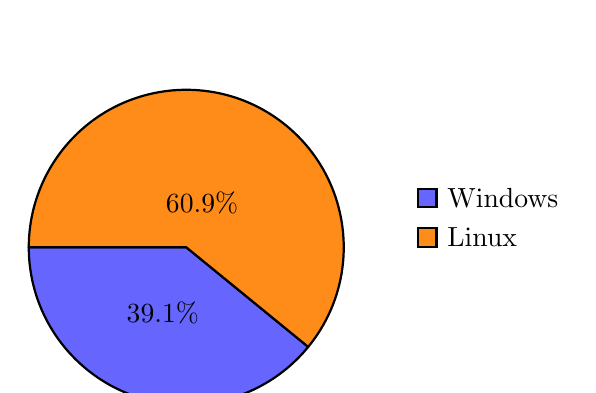
\begin{tikzpicture}
       \pie [rotate = 180, color = {blue!60, orange!90}, radius = 2, text = legend]
   {39.1/Windows,
    60.9/Linux}
 
   \end{tikzpicture}
 
   \cite{form}


   I den första frågar i formuläret så fick vi reda på att 60.0\% av 23 svar, ansåg att Linux skulle ha högre prestanda en Windows.

    \vspace{.5cm}
    Vi lät även deltagare att motiviera sina åtankar (inte obligatoriskt). Ett mycket välmotiverat svar: \begin{displayquote}I don't have much, just wanted to say that linux will ofc perform better in day to day tasks due to the fact that it consumes less resources in the first place

    on another note, let the numbers speak by themselfs \hyperlink{https://www.phoronix.com/scan.php?page=article&item=win10-debian101-intel} [\dots] just in general, the flexivility that linux provides is the main reason it performs better, as you can fit it much better to the job to have the maximum performance of your hardware

    the way you compile the kernel can drastically change the performance of linux over an application, this can depend on the architecture and instructions you use to compile, small tweaks like buffer sizes to allow for better scalability on very high core count cpu's, the compiler you use like ICC for intel, AOCC for Amd, Clang, GCC, etc...
    \end{displayquote}

Det här svaret från en av applikanterna är lik och en del av min egen hypotes (läs mer om detta på sida: \pageref{slutsatts})


   \vspace{3cm}
 
   \large{If you had the option to choose between Windows and Linux which one would you choose? (of course, you can choose any distro for Linux)}
  
   \vspace{.5cm}
  
   \normalsize I Denna fråga så frågar vi utvecklare vilket operativsystem dom skulle välja om dom hade chansen. Vi fick ett ganska fascinerande resultat. Om vi hade fått ett jämt antal svar så hade det varit en rak 50 50 på denna fråga men den tjugotredje personen som svarade på frågan valde Linux över Windows.
 
   \vspace{1cm}
 
   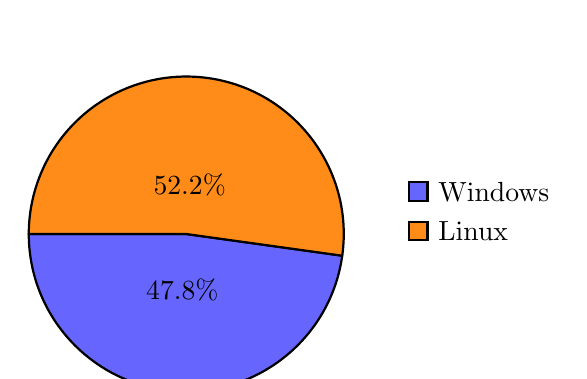
\begin{tikzpicture}
       \pie [rotate = 180, color = {blue!60, orange!90}, radius = 2, text=legend]
   {47.8/Windows,
    52.2/Linux}
 
   \end{tikzpicture}
 
   \cite{form}
 
   \vspace{1cm}

   \subsection{Prestanda skillnader}

   \subsubsection{Linux}
   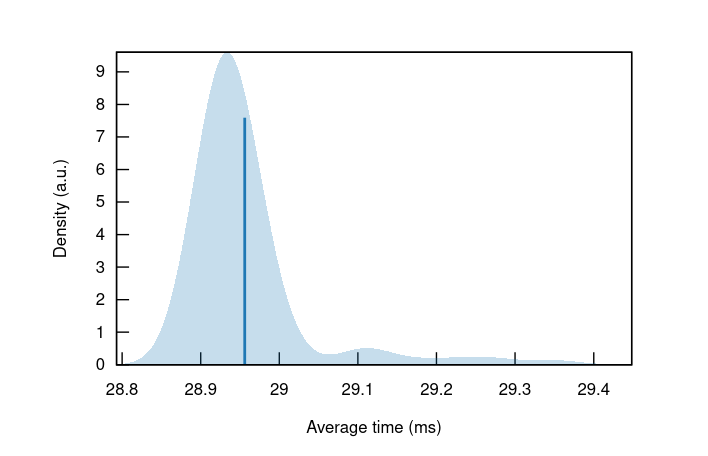
\includegraphics[width=1\textwidth]{bench_linux_average_time}


\section{Analys/diskussion}

\subsection{Formulär}

\subsubsection{Fråga 1}
Den första frågan var inom förväntningar. Anledningen till detta är att alla utväcklare inte känner till Linux på en djupare nivå än att Ubuntu är en av dom vanligasta distrobutionerna\cite{commondistro}.

\subsubsection{Fråga 2}
Den andra frågan var däremot ganska fårvånande i och med att 52.5\% av som svarde skulle välja Linux över Windows om dom hade chansen. Detta är ganska förbryllande eftersom att Linux är välkänt för att kräva mycket konfiguration och eller datorintresse. Man kan tänka sig att många utvecklare skulle vara högt dator intresserade men det är inte sant (enligt min upplevelse i och kring forum). Många frontend utvecklare använder sig of ta av proprietära program som Adobe Experience Design (Adobe Xd). 

\subsection{Problem med metodiken}

\subsubsection{Formuläret och vinklad data}

Vinklad data kan och formodligen är ett problem med formuläret som jag har skickat ut. Anledningen bakom det vinklade datan som jag har fått ut av formuläret är ställena jag har skickat ut det. Jag har skickat formuläret på design/web/programmerings relaterade forum och även skickade det via min mor som är team leader för en grupp utväcklare. Om jag hade skickat formuläret på andra mer publika medium så hade förmodligen datan sätt mycket annorlunda ut eftersom att manjoriteten av befolkning inte känner till Linux även dock det finns över allt runt om kring os. Dom finns i våra telefoner, datorerer, klockor, mm.


\section{Slutsats}\label{slutsatts}



\printbibliography


\end{document}


%% Note to self:

%% Write about how Linux stays ahead in security and performance by switching to newer versions of File systems and other systems/software.